%\documentclass[border=5pt,tikz]{standalone}
%\usetikzlibrary{positioning}
%\begin{document}
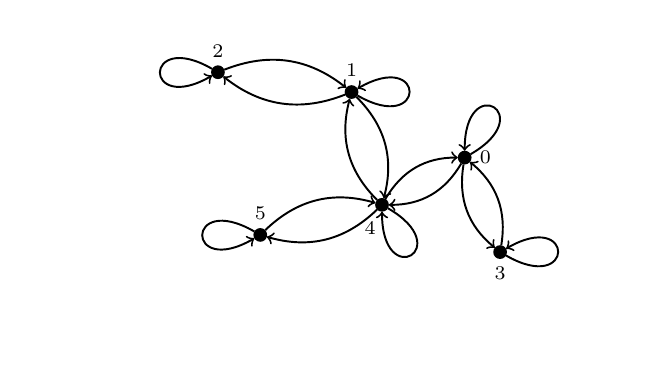
\begin{tikzpicture}[dot/.style={draw,circle,fill,inner sep=1.5pt},line width=.7pt,x=1.5cm,y=1.5cm]
\clip(-1,.8) rectangle (4,3.5);
\begin{scriptsize}
\node[label=right:0] (r0) at (2.7,2.4) [dot] {};

\node[label=above:1] (r1) at (1.7420645075484014,2.9548225063123694) [dot] {};
%\draw[color=black] (1.8316581320147085,3.195605372065557) node {$1$};


\node[label=above:2] (r2) at (0.6109449986613309,3.1228105521866865) [dot] {};
%\draw[color=black] (0.7005386231276353,3.363593417939874) node {$2$};

\node[label=below:3] (r3) at (3,1.6) [dot] {};
%\draw[color=black] (2.6,1.2357448368651927) node {$3$};

\node (r4) at (2,2) [dot] {};
\draw[color=black] (1.9,1.8) node {$4$};

\node[label=above:5] (r5) at (0.9693194965265414,1.7453085760172875) [dot] {};
%\draw[color=black] (1,2) node {$5$};

\draw[->] (r0) to[out=30,in=90,looseness=30] (r0);
\draw[->] (r1) to[out=-30,in=30,looseness=30] (r1);
\draw[->] (r2) to[out=150,in=210,looseness=30] (r2);
\draw[->] (r3) to[out=-30,in=30,looseness=30] (r3);
\draw[->] (r4) to[out=-30,in=-90,looseness=30] (r4);
\draw[->] (r5) to[out=150,in=210,looseness=30] (r5);

\draw[->] (r0) to[bend left] (r4);
\draw[->] (r4) to[bend left] (r0);

\draw[->] (r0) to[bend right] (r3);
\draw[->] (r3) to[bend right] (r0);

\draw[->] (r5) to[bend left] (r4);
\draw[->] (r4) to[bend left] (r5);

\draw[->] (r1) to[bend left] (r4);
\draw[->] (r4) to[bend left] (r1);

\draw[->] (r1) to[bend left] (r2);
\draw[->] (r2) to[bend left] (r1);

\end{scriptsize}
\end{tikzpicture}
%\end{document}
